\chapter{Administración remota}

En informática no siempre tenemos los equipos que administramos en nuestra oficina. Pueden estar en otro edificio, la oficina de un cliente, en internet … por lo tanto no siempre es posible acceder de manera física a ellos, y por tanto entra en juego la \textbf{administración remota}.

Podemos definir la administración remota como el sistema que nos permite realizar ciertas acciones “lanzadas” desde nuestro equipo local pero que serán ejecutadas en un equipo remoto.

Se pueden diferenciar dos tipos de sistemas dentro de la administración remota:

\begin{itemize}
    \item \textbf{Ejecución remota}: Lanzamos la acción a ejecutar desde un equipo remoto a través de algún tipo de interfaz o comando (que viajará a través de un protocolo securizado) y esperaremos a la respuesta.

    \item \textbf{Acceso remoto}: En este caso lo que hacemos es conectarnos al equipo a través de un protocolo que nos va a permitir administrarlo como si estuviésemos delante de él.
\end{itemize}

Ambos sistemas pueden ser complementarios, y puede que podamos administrar un mismo sevicio de ambas maneras, por lo que queda a nuestra disposición elegir el mejor método en cada momento.

Por otro lado, dependiendo de qué tipo de administración vayamos a llevar a cabo, o el protocolo que utilice, tendremos que tener acceso al servidor de alguna manera (ya sea conexión directa o mediante VPN).

\infobox{\textbf{Dependiendo de la administración remota que realicemos, necesitaremos conexión directa o mediante VPN al equipo que nos queremos conectar.}}

Por último, también debemos de conocer el tipo de protocolo que vamos a utilizar al realizar la conexión remota y por dónde va a pasar esa comunicación. Siempre hay que premiar la seguridad de la comunicación, y más cuando esta puede pasar por redes no controladas. Por lo tanto, deberemos asegurar que el protocolo utilizado es seguro, o en caso contrario, securizarlo de alguna manera.

\errorbox{\textbf{Siempre debemos confirmar que la comunicación que se realiza para la administración remota viaja cifrada.}}

Más adelante veremos cómo securizar una comunicación no segura realizando un túnel mediante el protocolo SSH en entornos GNU/Linux.


\section{Ejecución remota}

Este sistema de administración permite enviar acciones al equipo remoto a través de un protocolo establecido, y  dependiendo de la acción ejecutada se esperará una respuesta o no.

\begin{center}
    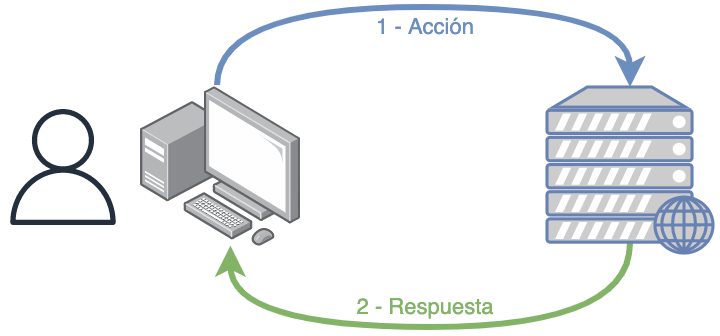
\includegraphics[width=0.7\linewidth]{ejecucion_remota.png}
\end{center}

Hoy en día es muy habitual este tipo de sistemas a través de disintos \textbf{CLI} (\textit{client line interface})  o \textbf{GUI} (\textit{graphic user interface}) que nos permiten administrar servicios remotos. Por ejemplo:

\begin{itemize}
    \item \textbf{\href{https://aws.amazon.com/es/cli/}{AWS CLI}}: Es el interfaz de línea de comandos para poder administrar de manera remota los servicios contratados en la nube AWS de Amazon.

    \item \textbf{\href{https://cloud.google.com/cli}{Gcloud CLI}}: Similar al caso anterior pero esta vez para Google Cloud.

    \item \textbf{\href{https://www.microsoft.com/en-us/download/details.aspx?id=45520}{Remote Server Administration Tools for Windows 10}}: En este caso se trata de un interfaz gráfico (\textbf{GUI}) que nos permite administrar un Windows Server desde un equipo Windows 10.
\end{itemize}

En los dos primeros ejemplos, al tratarse de servicios ofrecidos por un proveedor, hacen uso de un sistema de protocolo basado en conexión HTTPS.

Antes de poder realizar las ejecuciones deberemos configurar un sistema de autenticación para que el servicio remoto acepte las peticiones enviadas. En algunos casos será usando unos sistemas de certificados y en otros introduciendo un usuario y contraseña que establecerá una sesión temporal.

En los dos primeros ejemplos no nos estamos conectando directamente a nuestros servidores alojados en esas nubes, si no que lanzamos la orden a un “proxy” que verificará nuestros credenciales, verá los permisos que tenemos y después realizará la acción solicitada.


%TODO: mirar algo de esto
%COSAS A MIRAR:
%
%
%ADmin center
%
%https://learn.microsoft.com/en-us/windows-server/manage/windows-admin-center/plan/installation-options
%
%sconfig en windows    https://learn.microsoft.com/en-us/windows-server/administration/server-core/server-core-sconfig
%
%
%diferencias entre windows server core and escritorio https://learn.microsoft.com/en-us/windows-server/get-started/install-options-server-core-desktop-experience


\section{Acceso remoto}
Este sistema permite acceder al sistema y podremos administrarlo como si nos encontrásemos delante. Dependiendo del sistema la conexión nos permitirá interactuar de alguna de las siguientes maneras:

\begin{itemize}
    \item \textbf{CLI}: Mediante una conexión de línea de comandos. Es el caso más habitual en servidores GNU/Linux y la conexión se hace a través del protocolo seguro \textbf{SSH}.

    \item \textbf{GUI}: Podremos obtener un interfaz gráfico con el que veremos lo que está ocurriendo en pantalla en ese momento. En este caso, dependiendo del sistema, existirán distintas opciones, pero vamos a nombrar dos de ellas:

    \begin{itemize}
        \item \textbf{RDP}: Es el protocolo de escritorio remoto de Microsoft que transmite la información gráfica que el usuario debería ver por la pantalla, la transforma en el formato propio del protocolo, y la envía al cliente conectado. El problema es que este sistema desconecta al usuario que está logueado para poder hacer uso del escritorio remoto.

        \item \textbf{VNC}: En inglés \textit{Virtual Network Computing}, es un servicio con estructura \textbf{cliente-servidor} que permite visualizar el escritorio del servidor desde un programa cliente. En este caso, no existe desconexión del usuario que está logueado y por tanto podrá ver lo que le están realizando de manera remota.

        Es muy habitual que los equipos de usuarios ya tengan la instalación del servidor hecha, para que de esta manera, en caso de incidencia, poder realizar la conexión remota sin que el usuario tenga que realizar ninguna acción.
    \end{itemize}
\end{itemize}




\clearpage